\section{Analysis strategy}

Now that everything is set up and running, let us dive into the exercise! This tutorial uses data collected at the CMS experiment during the \texttt{Run2} data taking period (2017). The data is stored in \texttt{NanoAOD} files, version 9. You can find more information about the datasets in the folder  \code{campaign\_2017\_nano\_v9} located at \texttt{modules/cmsdb/cmsdb/campaings}. The first step is to retrieve these datasets using their \texttt{Logical File Names (LFNs)}. For this you can run the following command:
\begin{lstlisting}[language=bash]
law run cf.GetDatasetLFNs --processes h_ggf_4l --datasets h_ggf_4l_powheg
\end{lstlisting}

The datasets are now available and we are ready to start looking for the Higgs.  We will do this in several steps. 

\begin{itemize}
\item he first step is to implement a \underline{lepton selection} such that we are only left with events containing four leptons in the final state (i.e. either two $e^+e^-$ pairs,  two $\mu^+\mu^-$ pairs, or one $e^+e^-$ and $\mu^+\mu^-$ pair). This lepton selection is applied by writing a \CCSPStlye{Selector} object (section \ref{selector}). At this step, we can also implement \underline{kinematic cuts}, \underline{vertex cuts}, \underline{Isolation \& ID criteria} and \underline{trigger selections}.  The \CCSPStlye{Selector} will filter out events containing physics object which do not fulfil all of these criteria.

\item The second step will be to reconstruct the invariant mass of the four leptons so that we can find plausible $Z$ candidates. This is done by writing a \CCSPStlye{Producer} object (section \ref{producer}). This object will calculate the invariant mass and produce a new column to store this information for each event which passed the selection criteria mentioned above.

\item 

\end{itemize}

\begin{figure}[!h]
    \centering
    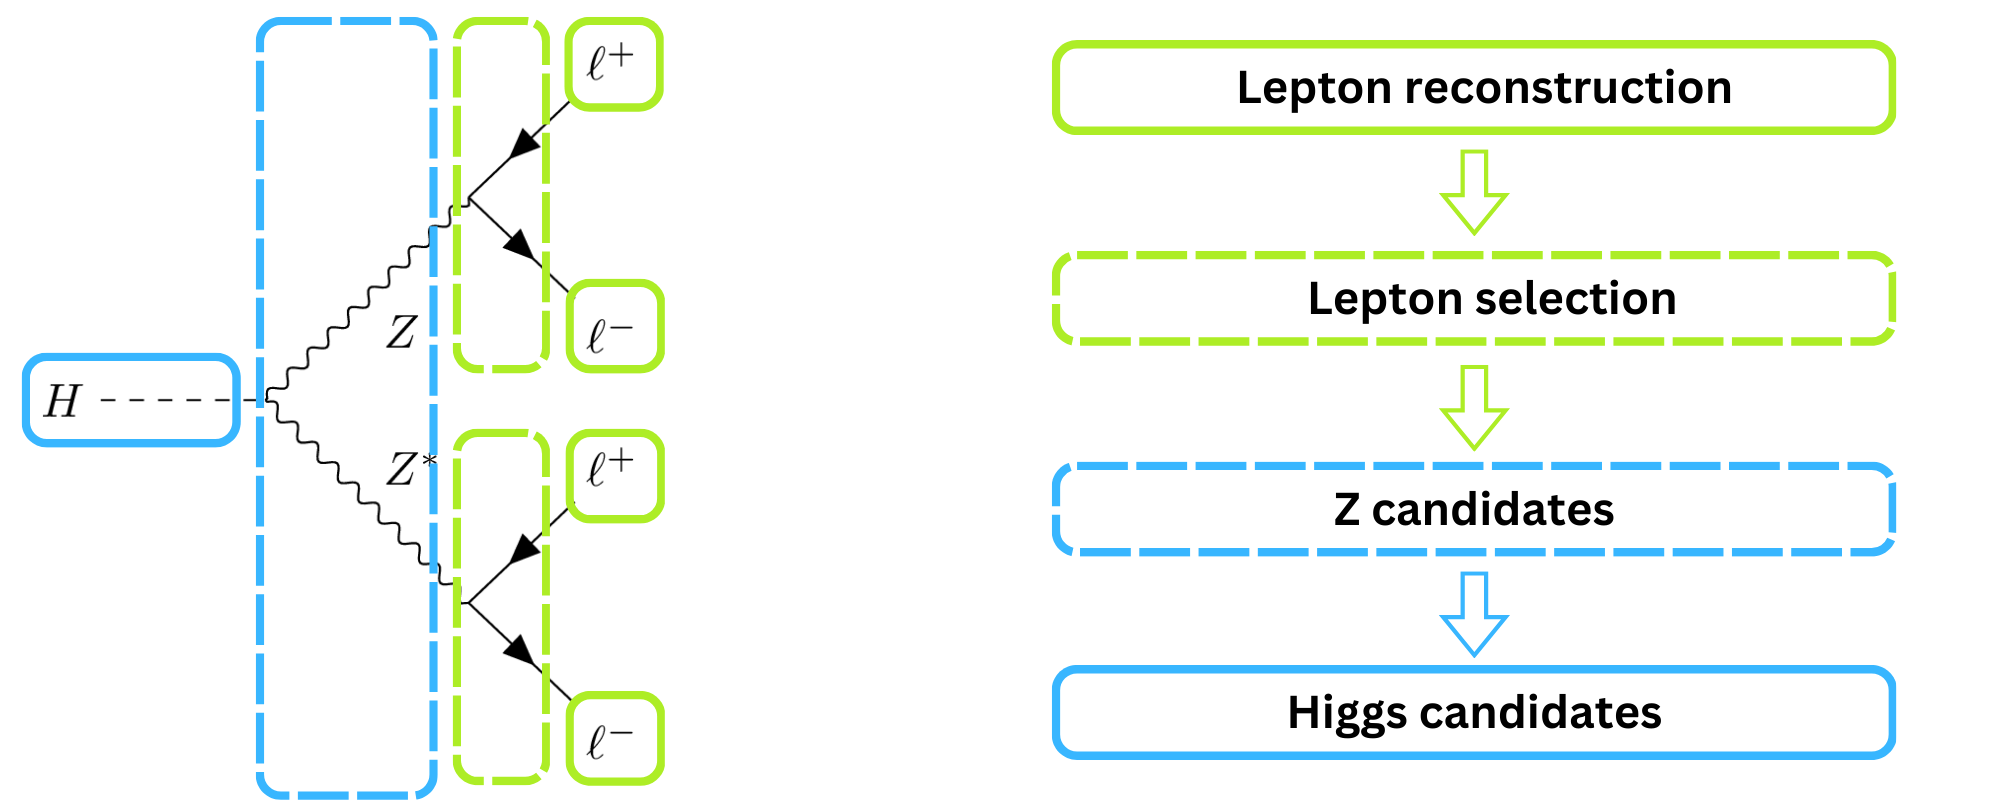
\includegraphics[scale=0.62]{images/strategy.png}
\end{figure}